% This file was created with tikzplotlib v0.10.1.
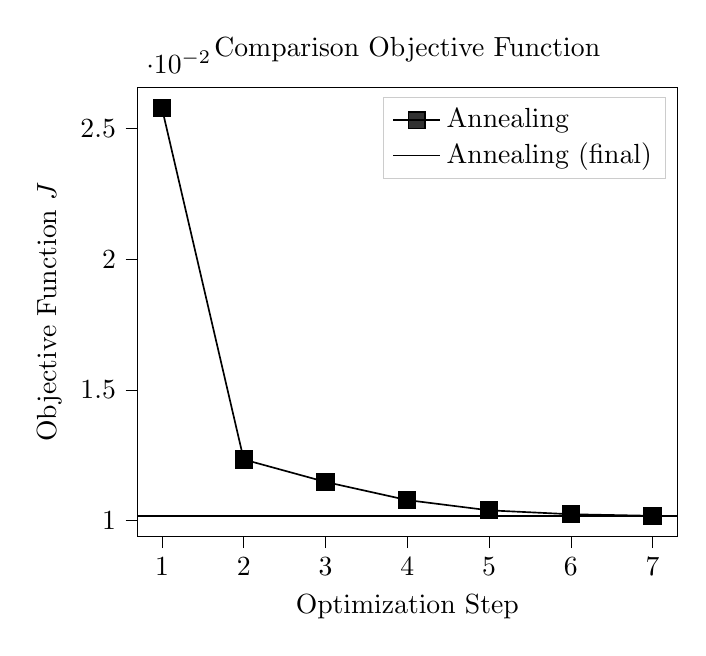
\begin{tikzpicture}

\definecolor{darkgray176}{RGB}{176,176,176}
\definecolor{lightgray204}{RGB}{204,204,204}

\begin{axis}[
legend cell align={left},
legend style={fill opacity=0.8, draw opacity=1, text opacity=1, draw=lightgray204},
tick align=outside,
tick pos=left,
title={Comparison Objective Function},
x grid style={darkgray176},
xlabel={Optimization Step},
xmin=0.7, xmax=7.3,
xtick style={color=black},
y grid style={darkgray176},
ylabel={Objective Function \(\displaystyle J\)},
ymin=0.00940254719344663, ymax=0.0265537128729074,
ytick style={color=black}
]
\addplot [semithick, black, mark=square*, mark size=3, mark options={solid}]
table {%
1 0.0257741144329319
2 0.0123369802818659
3 0.0114793317682522
4 0.0107845092471098
5 0.0103921655138229
6 0.0102422753718429
7 0.0101821456334221
};
\addlegendentry{Annealing}
\addplot [semithick, black]
table {%
0.7 0.0101821456334221
7.3 0.0101821456334221
};
\addlegendentry{Annealing (final)}
\end{axis}

\end{tikzpicture}
